% Created 2013-05-23 Thu 09:29
\documentclass{article}
\usepackage{epcc}
\usepackage{hyperref}

\title{Sharpen Exercise\\Using HPC resources and running parallel applications}
\author{Andrew Turner, Dominic Sloan-Murphy, David Henty, Adrian Jackson}
% \date{21 April 2014}
\begin{document}
\makeEPCCtitle

\setcounter{tocdepth}{3}
\tableofcontents
% \vspace*{1cm}

\section{Aims}
\label{sec-1}


The aim of this exercise is to get you used to logging into an HPC
resource, using the command line and an editor to manipulate files,
and using the batch submission system.
We will be using ARCHER for this exercise.  ARCHER is the UK national
HPC service, and is a Cray XC30 system with a total of 118,010 cores
(4920 nodes).

You can find more details on ARCHER and how to use it in the User
Guide at:

\begin{itemize}
\item \href{http://www.archer.ac.uk/documentation/user-guide/}{http://www.archer.ac.uk/documentation/user-guide/}
\end{itemize}
\section{Introduction}
\label{sec-2}


In this exercise you will run a simple program, in serial and
parallel, to sharpen the provided image.

Using your provided guest account, you will:

\begin{enumerate}
\item log onto the ARCHER frontend nodes;
\item copy the source code from a central location to your account;
\item unpack the source code archive;
\item compile the source code to produce an executable file;
\item run a serial job on the login node;
\item submit a serial job to the compute nodes using the PBS batch system;
\item submit a parallel job using the PBS batch system;
\item run the parallel executable on using an
   increasing number of cores and examine the performance improvement.
   
\end{enumerate}

Demonstrators will be on hand to help you as required. Please
do ask questions if you do not understand anything in the 
instructions - this is what the demonstrators are here for.
\section{Instructions}
\label{sec-3}
\subsection{Log into ARCHER frontend nodes and run commands}
\label{sec-3-1}


You should have been given a guest account ID -- referred to
generically here as \verb+guestXX+ -- and password. If you have not,
please contact a demonstrator.

\subsubsection{Procedure for Mac and Linux users}
\label{sec-3-1-1}


Open a command line \emph{Terminal} and enter the following command:


\begin{verbatim}
  user@laptop$ ssh -X guestXX@login.archer.ac.uk
  Password:
\end{verbatim}

you should be prompted to enter your password.
\subsubsection{Procedure for Windows users}
\label{sec-3-1-2}

Windows does not generally have SSH installed by default so some extra
work is required. You need to download and install a SSH client
application - PuTTY is a good choice:

\begin{itemize}
\item \href{http://www.chiark.greenend.org.uk/~sgtatham/putty/}{http://www.chiark.greenend.org.uk/\textasciitilde sgtatham/putty/.}
\end{itemize}

When you start PuTTY you should be able to enter the ARCHER login
address (login.archer.ac.uk). When you connect you will be prompted
for your username and password.

You can follow the instructions for setting up PuTTY by watching the
introductory video
here:\\ \href{https://www.youtube.com/watch?v=oVFQg1qFjKQ}{https://www.youtube.com/watch?v=oVFQg1qFjKQ}

By default, PuTTY does not send graphics back to your local
machine. We will need this later for viewing the sharpened image, so
you should ``Enable X11 Forwarding'' which is an option in the
``Category'' menu under ``Connection -> SSH -> X11''. You will need to
do this each time before you log in with PuTTy.

\subsection{Running commands}
\label{sec-3-2}


You can list the directories and files available by
using the \emph{ls} (LiSt) command:


\begin{verbatim}
  guestXX@archer:~> ls
  bin  work
\end{verbatim}

NB: The first time you do this there will be no files or directories
so 'ls' will return with an empty line.

You can modify the behaviour of commands by adding options. Options
are usually letters or words preceded by `-'. For example,
to see more details of the files and directories available you can
add the `-l' (l for long) option to \emph{ls}:


\begin{verbatim}
  guestXX@archer:~> ls -l
  total 8
  drwxr-sr-x 2 user z01 4096 Nov 13 14:47 bin
  drwxr-sr-x 2 user z01 4096 Nov 13 14:47 work
\end{verbatim}

If you want a description of a particular command and the options
available you can access this using the \emph{man} (MANual) command. 
For example, to show more information on \emph{ls}:


\begin{verbatim}
  guestXX@archer:~> man ls
  Man: find all matching manual pages
   * ls (1)
     ls (1p)
  Man: What manual page do you want?
  Man:
\end{verbatim}

In the manual, use the spacebar to move down, `u' to move up,
and `q' to quit to the command line.


\subsection{Download and extract the exercise files}
\label{sec-3-5}


Firstly, change directory to make sure you are on the ``/work''
filesystem on ARCHER.

\begin{verbatim}
  guestXX@archer:~> cd /work/y14/y14/guestXX/
\end{verbatim}

/work is a high performance parallel file system that can be accessed
by both the frontend and compute nodes. \textbf{All jobs on ARCHER
  should be run from the /work filesystem.} ARCHER compute nodes
cannot access the /home filesystem at all. Any jobs attempting to use
/home will fail with an error.

Use \emph{wget} (on ARCHER) to get the exercise files archive from the
EPCC webserver. Material for the courses is stored in a standard
location of the form:

\begin{verbatim}
  http://www.archer.ac.uk/training/course-material/YYYY/MM/CourseName_Location/.
\end{verbatim}

If you access the material with a web browser it will be
downloaded to your laptop, which is not very useful if we want the
files on ARCHER. It is easier to copy them straight from the
website to ARCHER:

\begin{verbatim}
  guestXX@archer:~> wget http://www.archer.ac.uk/.../Exercises/sharpen.tar.gz
  --2014-06-27 16:15:42--  http://www.archer.ac.uk/training/course-material/2014/06/IntroHPC_Edi/Exercises/sharpen.tar.gz
  Resolving www.archer.ac.uk... 193.62.216.12
  Connecting to www.archer.ac.uk|193.62.216.12|:80... connected.
  HTTP request sent, awaiting response... 200 OK
  Length: 1754173 (1.7M) [application/x-gzip]
  Saving to: `sharpen.tar.gz'

  100%[======================================>] 1,754,173   --.-K/s   in 0.02s   

  2014-06-27 16:15:42 (107 MB/s) - `sharpen.tar.gz.1' saved [1754173/1754173]
\end{verbatim}

To unpack the archive:

\begin{verbatim}
  guestXX@archer:~> tar -xzvf sharpen.tar.gz
  sharpen/C-SER/
  sharpen/C-SER/filter.c
  ...
  --snip--
  ...
  sharpen/F-OMP/dosharpen.f90
  sharpen/F-OMP/Makefile
  sharpen/F-OMP/fuzzy.pgm
\end{verbatim}

 If you are interested in the C examples move to the
\emph{C-SER} subdirectory; for Fortran, move to \emph{F-SER}. For example:

\begin{verbatim}
  guestXX@archer:~> cd sharpen/C-SER
\end{verbatim}

\subsection{Using the Emacs text editor}
\label{sec-3-3}


Running interactive graphical applications on ARCHER can be very slow.
It is therefore best to use Emacs will be used in \emph{in-terminal}
mode. In this mode you can edit the file as usual but you must use
keyboard shortcuts to run operations such as ``save file'' (remember,
there are no menus that can be accessed using a mouse).

Start Emacs with the \emph{emacs -nw} command and the name of the file
you wish to edit or create. For example:


\begin{verbatim}
  guestXX@archer:~> emacs -nw sharpen.pbs
\end{verbatim}

The terminal will change to show that you are now inside the Emacs
text editor:

{\centerline{\resizebox{0.70\hsize}{!}{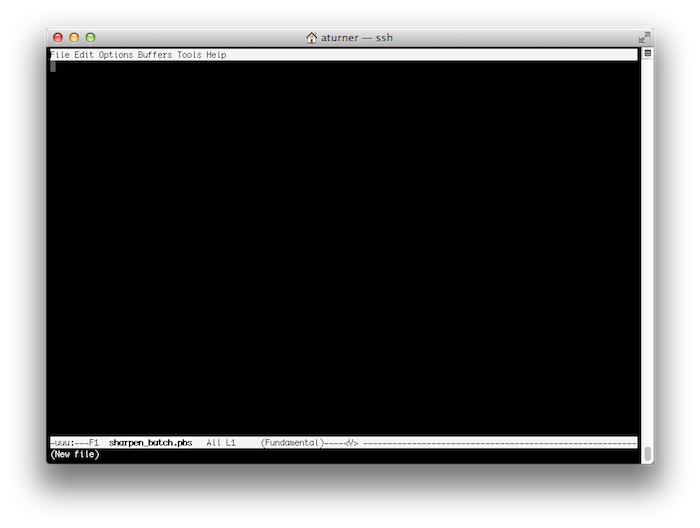
\includegraphics{emacs_terminal.png}}}}

Typing will insert text as you would expect and backspace will delete
text. You use special key sequences (involving the Ctrl and Alt
buttons) to save files, exit Emacs and so on.

Files can be saved using the sequence ``Ctrl-x Ctrl-s'' (usually
abbreviated in Emacs documentation to ``C-x C-s''). You should see the
following briefly appear in the line at the bottom of the window (the
minibuffer in Emacs-speak):


\begin{verbatim}
  Wrote ./sharpen.pbs
\end{verbatim}

To exit Emacs and return to the command line use the sequence ``C-x
C-c''. If you have changes in the file that have not yet been saved
Emacs will prompt you (in the minibuffer) to ask if you want to save
the changes or not.

Although you could edit files on your local machine using whichever
windowed text editor you prefer it is useful to know enough to use an
in-terminal editor as there will be times where you want to perform a
quick edit that does not justify the hassle of editing and
re-uploading.

\subsection{Useful commands for examining files}
\label{sec-3-4}


There are a couple of commands that are useful for displaying the
contents of plain text files on the command line that you can use to
examine the contents of a file without having to open in in Emacs (if
you want to edit a file then you will need to use Emacs). The commands
are \emph{cat} and \emph{less}. \emph{cat} simply prints the contents of the file to
the terminal window and returns to the command line. For example:


\begin{verbatim}
  guestXX@archer:~> cat sharpen.pbs
  ...
\end{verbatim}

This is fine for small files where the text fits in a single terminal
window. For longer files you can use the \emph{less} command: \emph{less} gives
you the ability to scroll up and down in the specified file. For
example:

\begin{verbatim}
  guestXX@archer:~> less Makefile
\end{verbatim}

Once in \emph{less} you can use the spacebar to scroll down and `u' to
scroll up. When you have finished examining the file you can use `q'
to exit \emph{less} and return to the command line.



This program takes a fuzzy image and uses a simple algorithm to
sharpen the image. A very basic parallel version of the algorithm has
been implemented which we will use in this exercise.  There are a
number of versions of the sharpen program available:

\begin{description}
\item[C-SER] Serial C version
\item[F-SER] Serial Fortran version
\item[C-MPI] Parallel C version using MPI
\item[F-MPI] Parallel Fortran version using MPI
\item[C-OMP] Parallel C version using OpenMP
\item[F-OMP] Parallel Fortran version using OpenMP

\end{description}
\subsection{Compile the source code to produce an executable file}
\label{sec-3-6}

We will first compile the serial version of the code for our
example.

\begin{verbatim}
  guestXX@archer:~> ls
  cio.c        filter.c   Makefile   sharpen.h    utilities.c
  dosharpen.c  fuzzy.pgm  sharpen.c  sharpen.pbs  utilities.h

  guestXX@archer:~> make
  cc -g -DC_SERIAL_PRACTICAL -c sharpen.c
  cc -g -DC_SERIAL_PRACTICAL -c dosharpen.c
  cc -g -DC_SERIAL_PRACTICAL -c filter.c
  cc -g -DC_SERIAL_PRACTICAL -c cio.c
  cc -g -DC_SERIAL_PRACTICAL -c utilities.c
  cc -g -DC_SERIAL_PRACTICAL -o sharpen sharpen.o dosharpen.o filter.o cio.o utilities.o -lm

 guestXX@archer:~> 
\end{verbatim}

This should produce an executable file called \emph{sharpen} which we
will run on ARCHER.

For the Fortran version, the process is exactly the same as above,
except you should move to the \emph{F-SER} subdirectory and build the
program there:

\begin{verbatim}
  guestXX@archer:~> cd sharpen/F-SER
  guestXX@archer:~> make
  ...
\end{verbatim}

As before, this should produce a \emph{sharpen} executable.

Don't worry about the C file \verb+utilities.c+ -- it is just
providing an easy method for printing out various information about
the program at run time, and it is most easily implemeted in C.

\subsection{Running a serial job}

You can run this serial program directly on the login nodes, e.g.:

\begin{verbatim}
  guestXX@archer:~> ./sharpen
  Image sharpening code running in serial

  Input file is: fuzzy.pgm
  Image size is 564 x 770

  Using a filter of size 17 x 17

  Reading image file: fuzzy.pgm
  ... done

  Starting calculation ...
  On core 0-31
  ... finished

  Writing output file: sharpened.pgm

  ... done

  Calculation time was 5.579000 seconds
  Overall run time was 5.671895 seconds
\end{verbatim}

\subsection{Viewing the images}

To see the effect of the sharpening algorithm, you can view the images
using the {\verb+display+} program from the ImageMagick suite.

\begin{verbatim}
  guestXX@archer:~> display fuzzy.pgm
  guestXX@archer:~> display sharpened.pgm
\end{verbatim}

Type ``q'' in the image window to close the program.

To view the image you will need an X window client installed.  Linux
or Mac systems will generally have such a program available, but
Windows does not provide X windows functionality by default.  There
are many X window systems available to install on Windows; we
recommend Xming available at:

\begin{itemize}
\item \href{http://sourceforge.net/projects/xming/}{http://sourceforge.net/projects/xming/}
\end{itemize}

\subsection{Running on the compute nodes}
\label{sec-3-7}

As with other HPC systems, use of the compute nodes on ARCHER is mediated by the PBS
job submission system. This is used to ensure that all users get access to
their fair share of resources, to make sure that the machine is as
efficiently used as possible and to allow users to run jobs without
having to be physically logged in.

Whilst it is possible to run interactive jobs (jobs where you log directly into the backend nodes on ARCHER and run your executable there) on ARCHER, and they are useful for debugging and development,
they are not ideal for running long and/or large numbers of production
jobs as you need to be physically interacting with the system to use
them.

The solution to this, and the method that users generally use to run jobs on systems like ARCHER, is to run in \emph{batch} mode. In this case you put
the commands you wish to run in a file (called a job script) and the
system executes the commands in sequence for you with no need for you
to be interacting.

\subsubsection{Using PBS job scripts}
\label{sec-3-7-1}


We will first run the same serial program on the compute nodes.
Look at the batch script:

\begin{verbatim}
  guestXX@archer:~> emacs sharpen.pbs
\end{verbatim}

The first line specifies which \emph{shell} to use to interpret the commands we
include in the script. Here we use the Bourne Again SHell (bash) which is
the default on most modern systems. The --login option tells the shell to
behave as if it was an interactive shell.

 The line \emph{-l select=[nodes]} is used to request
the total number of compute nodes required for your job (1 in the example
above).

The \#PBS lines provide options to the job submission system where
``-l select'' specifies that we want to reserve 1 compute node for
our job - the minimum job size on ARCHER is 1 node (24 cores); the
``-l walltime=00:01:00'' sets the maximum job length to 1 minute;
``-A y14'' sets the budget to charge the job to ``y14''; ``-N
sharpen'' sets the job name to ``sharpen''. 

The remaining lines are the commands to be executed in the job. Here
we have a comment beginning with ``\#'', a directory change to
\$PBS\_O\_WORKDIR (an environment variable that specifies the
directory the job was submitted from) and the aprun command (this
command tells the system to run the jobs on the compute nodes rather
than the frontend nodes).

Jobs can only be run on the compute nodes with the {\verb+aprun+}
parallel job launcher. The line
\begin{verbatim}
  aprun -n 1 ./sharpen
\end{verbatim}

runs a single copy of our serial executable.

\subsubsection{Submitting scripts to PBS}
\label{sec-3-7-2}

Simply use the qsub command and specify the special queue {\em
  course1} for your job; normally you do not specify a named queue on
ARCHER, but for courses we have reserved resources to enable faster
turnaround of jobs.


\begin{verbatim}
  guestXX@archer:~> qsub -q course1 sharpen.pbs
  58306.sdb
\end{verbatim}

The jobID returned from the \emph{qsub} command is used as part of the
names of the output files discussed below and also when you want to
delete the job (for example, you have submitted the job by mistake).

\subsubsection{Monitoring/deleting your batch job}
\label{sec-3-7-3}


The PBS command \emph{qstat} can be used to examine the batch queues and
see if your job is queued, running or complete. \emph{qstat} on its own
will list all the jobs on ARCHER (usually hundreds) so you can use the
``-u \$USER'' option to only show your jobs:


\begin{verbatim}
guestXX@archer:~> qstat -u $USER

sdb:
                                                            Req'd  Req'd   Elap
Job ID          Username Queue    Jobname    SessID NDS TSK Memory Time  S Time
--------------- -------- -------- ---------- ------ --- --- ------ ----- - -----
58306.sdb       guest01  standard sharpen       --    1  24    --  00:01 Q   --
\end{verbatim}

``Q'' means the job is queued, ``R'' that it is running and ``E'' that
it has recently completed; if you do not see your job, it usually
means that it has completed.

If you want to delete a job, you can use the \emph{qdel} command with the
jobID. For example:


\begin{verbatim}
  guestXX@archer:~> qdel 58306.sdb
\end{verbatim}
\subsubsection{Finding the output}
\label{sec-3-5-4}

The job submission system places the output from your job into two
files: <job name>.o<jobID> and <job name>.e<jobID> (note that the
files are only produced on completion of the job). The
sharpen.o<jobID> file contains the output from your job
sharpen.e<jobID> contains any errors.

\begin{verbatim}
  guestXX@archer:~> cat sharpen.o58306

  Image sharpening code running in serial

  Input file is: fuzzy.pgm
  Image size is 564 x 770

  Using a filter of size 17 x 17

  Reading image file: fuzzy.pgm
  ... done

  Starting calculation ...
  On core 0
  ... finished

  Writing output file: sharpened.pgm

  ... done

  Calculation time was 5.400482 seconds
  Overall run time was 5.496556 seconds
  Application 166570 resources: utime ~6s, stime ~0s, Rss ~18024, inblocks ~11176, outblocks ~13811
\end{verbatim}

\subsubsection{Extra exercise}

You could try running more than one copy of the
serial program by changing the ``-n'' argument to ``aprun''. What do you
observe?

%\subsection{Submit an interactive job and wait for it to start}
%\label{sec-3-8}
%
%As well as using the batch system to schedule and run your jobs, it is also possible to submit an \emph{interactive job}. An
%interactive job allows us to run executables on the ARCHER compute
%nodes directly from the command line using the \emph{aprun} command as we did in the batch script. This mode of use is extremely useful for
%debugging and code development as it allows you to get instant feed
%back on your executable on the compute nodes rather than having to
%wait for the end of the job (as is the case for non-interactive or
%\emph{batch} jobs). It has the disadvantage that you have to be physically
%logged into the machine to issue the commands.
%
%Submit an interactive job using the command (replace <resID> with the
%reservation ID provided by the trainer):
%
%
%\begin{verbatim}
%guestXX@archer:~> qsub -IV -l select=1,walltime=3:0:0 -A y14 -q <resID>
%qsub: waiting for job 57939.sdb to start
%\end{verbatim}
%
%(Note that there is no space between the select and walltime options
%above as they are both arguments to the ``-l'' option.) The meanings of
%the various options are:
%
%\begin{description}
%\item[-I] Interactive job
%\item[-V] Make the job environment match my current session
%\item[-l select=1] Reserve 1 node (24 cores) for this job.
%\item[-l walltime=3:0:0] Set a maximum wallclock time of 3 hours for
%     this job
%\item[-A y14] Charge the job to the y14 budget
%\item[-q <resID>] Submit the job in the specified reservation
%\end{description}
%
%
%The job may take a minute to start (or much longer if you are asking for larger numbers of nodes or longer job duration, one of the reasons that interactive jobs are not as convenient for production jobs as standard batch system jobs), when it starts you will be returned
%to a command prompt in your home directory.
%
%Once you have finished running executables on the compute nodes you
%can exit the interactive job using the \emph{exit} command (do not do this
%right now):
%
%\begin{verbatim}
%guestXX@mom3:~> exit
%logout
%
%qsub: job 57939.sdb completed
%\end{verbatim}
%
%If you type exit by mistake you can simply resubmit the job using the
%qsub command above again.
%
%\subsection{Run the parallel executable on a compute node}
%\label{sec-3-9}
%
%
%Firstly, change to the directory where you compiled the code. For
%example:
%
%
%\begin{verbatim}
%guestXX@mom3:~> cd /work/y14/y14/guestXX/sharpen/C-MPI
%guestXX@mom3:/work/y14/y14/guestXX/sharpen/C-MPI> ls
%Makefile  dosharpen.c  filter.o    location.h  sharpen.c  sharpen.pbs
%cio.c     dosharpen.o  fuzzy.pgm   location.o  sharpen.h
%cio.o     filter.c     location.c  sharpen     sharpen.o
%\end{verbatim}
%
%Use the \emph{aprun} command to run the sharpen executable using 4 parallel
%tasks - the `-n' option to \emph{aprun}  specifies how many
%parallel tasks to use:
%
%
%\begin{verbatim}
%guestXX@mom3:/work/y14/y14/guestXX/sharpen/C-MPI> aprun -n 4 ./sharpen
%
%Image sharpening code running on 4 processor(s)
%
%Input file is: fuzzy.pgm
%Image size is 564 x 770
%
%Using a filter of size 17 x 17
%
%Reading image file: fuzzy.pgm
%... done
%
%Starting calculation ...
%Process  0 is on cpu  0 on node nid02206
%Process  1 is on cpu  1 on node nid02206
%Process  2 is on cpu  2 on node nid02206
%Process  3 is on cpu  3 on node nid02206
%... finished
%
%Writing output file: sharpened.pgm
%
%... done
%
%Calculation time was 1.541406 seconds
%Overall run time was 1.602274 seconds
%Application 738180 resources: utime ~6s, stime ~0s, Rss ~24192, inblocks ~13693, outblocks ~17967
%\end{verbatim}
%
%If you try to run the executable using \emph{aprun} outwith an interactive
%job then you will see an error that looks like:
%
%
%\begin{verbatim}
%guestXX@archer:~> aprun -n 4 ./sharpen
%apsched: request exceeds max nodes, alloc
%\end{verbatim}

\subsection{Running a parallel job on the compute nodes}

Repeat the same procedure as above but use the parallel MPI version of
the code in \emph{C-MPI} or \emph{F-MPI}. By default, the batch
script is set up to run on 4 cores. You should see that that the
parallel code is faster than the serial one.

\section{Parallel Performance}

\subsection{Amdahl's law}

If you examine the log file you will see that it contains two timings:
the total time taken by the entire program (including IO) and the time
taken solely by the calculation. The image input and output is not
parallelised so this is a serial overhead, performed by a single
processor. The calculation part is, in theory, perfectly parallel
(each processor operates on different parts of the image) so this
should get faster on more cores.

You should do a number of runs and fill in Table~\ref{tab:timings}:
the IO time is the difference between the calculation time and the
overall run time; the total CPU time is the calculation time
multiplied by the number of cores. Note that if you run on more than
24 cores then you will need to request more than one node with the
''select='' option to PBS.

Look at your results -- do they make sense?  Given the structure of
the code, you would expect the IO time to be roughly constant, and the
performance of the calculation to increase linearly with the number of
cores: this would give a roughly constant figure for the total CPU
time. Is this what you observe?


The parallel speedup should closely follow Amdahl's law as the
calculation splits cleanly into a purely serial phase (IO) and a
perfectly parallel phase (calculation).

\subsection{OpenMP code}

If you are interested, you can try running the OpenMP code in
\emph{C-OMP} or \emph{F-OMP}.

Note that to change the number of cores that the program uses you must
set the environment variable \verb+OMP_NUM_THREADS+. This is already
done for you in the PBS script, although you will need to change the
actual number yourself.

Note that you can run using multiple threads on the login nodes -- you
must set \verb+OMP_NUM_THREADS+ before you run, e.g.:

\begin{verbatim}
  guestXX@archer:~> export OMP_NUM_THREADS=3 
  guestXX@archer:~> ./sharpen 

  Image sharpening code running on 3 thread(s)

  ...
\end{verbatim}

\begin{table}[h]
\begin{center}
\begin{tabular}{|c|l|l|l|l|}
\hline
\# Cores & Overall run time & Calculation time & IO time \ \ \ \ \
\ \ \ \
\ & Total
CPU time \\
\hline
\hline
1 & & & & \\
\hline
2 & & & & \\
\hline
4 & & & & \\
\hline
7 & & & & \\
\hline
10 & & & & \\
\hline
 & & & & \\
\hline
 & & & & \\
\hline
 & & & & \\
\hline
 & & & & \\
\hline
 & & & & \\
\hline
 & & & & \\
\hline
 & & & & \\
\hline
 & & & & \\
\hline
 & & & & \\
\hline
\end{tabular}
\begin{tabular}{|c|l|l|l|l|}
\hline
\# Cores & Overall run time & Calculation time & IO time \ \ \ \ \
\ \ \ \
\ & Total
CPU time \\
\hline
\hline
1 & & & & \\
\hline
2 & & & & \\
\hline
4 & & & & \\
\hline
7 & & & & \\
\hline
10 & & & & \\
\hline
 & & & & \\
\hline
 & & & & \\
\hline
 & & & & \\
\hline
 & & & & \\
\hline
 & & & & \\
\hline
 & & & & \\
\hline
 & & & & \\
\hline
 & & & & \\
\hline
 & & & & \\
\hline
\end{tabular}
\ \\
\begin{tabular}{|c|l|l|l|l|}
\hline
\# Cores & Overall run time & Calculation time & IO time \ \ \ \ \
\ \ \ \
\ & Total
CPU time \\
\hline
\hline
1 & & & & \\
\hline
2 & & & & \\
\hline
4 & & & & \\
\hline
7 & & & & \\
\hline
10 & & & & \\
\hline
 & & & & \\
\hline
 & & & & \\
\hline
 & & & & \\
\hline
 & & & & \\
\hline
 & & & & \\
\hline
 & & & & \\
\hline
 & & & & \\
\hline
 & & & & \\
\hline
 & & & & \\
\hline
\end{tabular}
\caption{\label{tab:timings} Time taken by parallel image processing code}
\end{center}
\end{table}

\end{document}
